\documentclass{article}
\usepackage[left=0.75in,top=0.6in,right=0.75in,bottom=0.6in]{geometry} %
\usepackage{graphicx}
\begin{document}
	\begin{center}
		%Name,Address,Contact information (Contact,e-mail), Photograph
		\vspace{10px}
	\textbf{\Huge ABHISHEK KUMAR VERMA}
   \line(3,0){500}\end{center}


\begin{flushleft}
 \begin{tabular}{l r}
 \textbf{\normalsize Mechanical Department}\hspace{190pt} & ~\textbullet~ {\textbf{\normalsize vermaabhishek357@gmail.com}}\\
 	\textbf{\normalsize PES Institute of Technology, Bengaluru-85 } \hspace{105pt} & ~\textbullet~ {\textbf{\normalsize 9738738157}}
 \end{tabular}   
  \end{flushleft}
 
\begin{figure}[h]
	\centering
\hspace{320pt}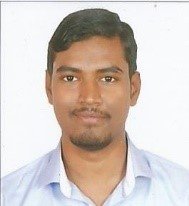
\includegraphics{pic.jpg}
\end{figure}


%OBJECTIVE

\begin{flushleft}\textbf{\LARGE OBJECTIVE}\\\vspace{10px}
	{\large To be associated with a company, where I can utilize my skills and make significant contribution to the organization and at the same time my individual growth.}\\\vspace{15px}
\end{flushleft}

	%EDUCATION

\textbf{\LARGE EDUCATION}\vspace{10px}\\\vspace{10px}
\begin{tabular}{|c|c|c|c|c|}\hline
	DEGREE & COLLEGE/SCHOOL & UNIVERSITY & PASSING YEAR & PERCENTAGE \\ \hline
	10th & Creane Memorial High School, Gaya & CBSE & 2010 & 93.1 \\ \hline
	12th & Jai Hind Public School, Gaya & CBSE & 2012 & 86.2 \\ \hline
	B.E. (Mech) & PES Institute of Technology, Bengaluru-85 & VTU & 2017 & 81.8 \\ \hline
\end{tabular}\vspace{15px}

%PROJECTS

\textbf{\LARGE PROJECTS}
\begin{enumerate}
	{\large \item •	Miniaturisation of Windmill to Utilize the Waste Wind Energy from Fans.}
	{\large \item • Line follower robot.}
	{\large \item •	Soccer playing robot.}
	{\large \item •	Remote Control Plane.}
	{\large \item •	Final Year Project : Design and Fabrication of Glass Wall Cleaning Robot.\\
		Presented this Robot Model at e-Yantra Ideas Competition, IIT Mumbai.}
\end{enumerate}\vspace{15px}

	%TRAINING AND INTERNSHIP

\textbf{\LARGE TRAINING AND INTERNSHIP}
\begin{itemize}
	{\large \item •	ROLON SEALS, Hyderabad. Topic – SolidWorks, AutoCAD and CNC Programming.}
	{\large \item •	TATA MOTORS (FOUNDRY DEPARTMENT), Jamshedpur. Project Topic- Study of optimum use of resources and increase productivity.}
\end{itemize}\vspace{15px}

	%TECHNICAL SKILLS

\textbf{\LARGE TECHNICAL SKILLS}
\begin{itemize}
	{\large \item CAD Software : Solid Edge, SolidWorks, AutoCAD 2D modelling, CATIAV5R20 }
	{\large \item CAE Software : Hyper Mesh}
	{\large \item MATLAB }
	{\large \item MS-office (Word, PowerPoint, Excel)}
\end{itemize}\vspace{15px}

	%SOFT SKILLS

\textbf{\LARGE SOFT SKILLS}
\begin{enumerate}
	{\large \item Critical observation and Problem solving }
	{\large \item Determined to learn with practical approach }
	{\large \item Teamwork and collaboration }
	{\large \item Flexibility }
	{\large \item Self-Motivation }
\end{enumerate}\vspace{15px}
	
\end{document}